\problemname{Godishalsbandet}
Alice vill dela ett godishalsband med Bob.
Halsbandet består av vita och blåa godisar.
För att vara rättvis vill Alice dela halsbandet i två
delar med lika många godisbitar i varje.
Dock gillar Alice de blåa godisarna mycket mer än de vita,
och vill därför få så många blåa godisar i sin halva som möjligt.

Vad är det största antalet blåa godisar Alice kan få i sin del,
om hon klipper halsbandet optimalt?

\section*{Indata}
Indatan består av en rad med en sträng som beskriver halsbandet.
Strängen består endast av bokstäverna \texttt{B} och \texttt{V},
och har totalt ett jämnt antal bokstäver.

\section*{Utdata}
Skriv ut en rad med ett heltal: det maximala antalet blåa godisar Alice
kan få i sin del av halsbandet.

\section*{Poängsättning}
Din lösning kommer att testas på en mängd testfallsgrupper.
För att få poäng för en grupp så måste du klara alla testfall i gruppen.

\noindent
\begin{tabular}{| l | l | p{12cm} |}
  \hline
  Grupp & Poängvärde & Gränser \\ \hline
  $1$   & $20$       & Halsbandet ser ut så som i figur \ref{fig:group-1}. \\ \hline
  $2$   & $40$       & Halsbandet består av högst $1\,000$ godisar. \\ \hline
  $3$   & $40$       & Inga ytterligare begränsningar. \\ \hline
\end{tabular}


\begin{figure}[h]
	\centering
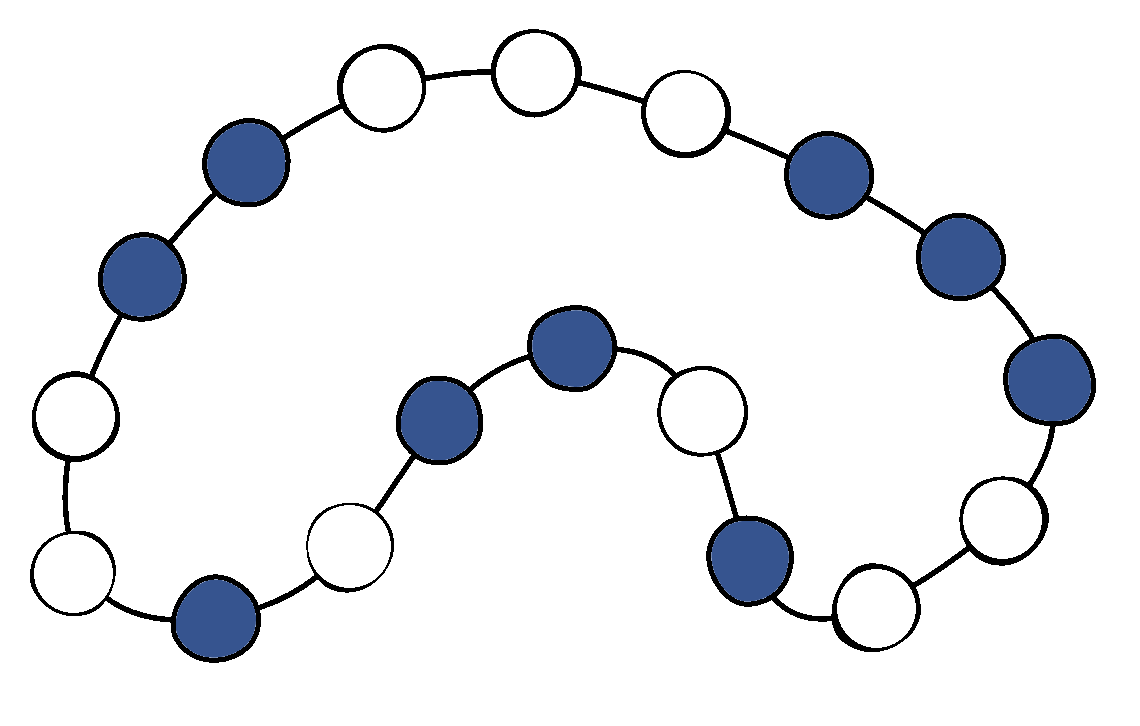
\includegraphics[width=0.5\textwidth]{group1}
\caption{Halsbandet i första testfallsgruppen}
\label{fig:group-1}
\end{figure}


\section*{Förklaring av exempelfall 1}
\texttt{BBVVBVVVBB} har längd 10 så Alice måste dela halsbandet i två delar med $5$ godisar i varje.
De möjliga delarna hon kan få är \texttt{BBVVB}, \texttt{BVVBV}, \texttt{VVBVV}, \texttt{VBVVV},
\texttt{BVVVB}, \texttt{VVVBB}, \texttt{VVBBB}, \texttt{VBBBB}, \texttt{BBBBV}, \texttt{BBBVV}.
Hon får mest blåa godisar genom att välja \texttt{VBBBB} eller \texttt{BBBBV} som har $4$ blåa godisar.



\begin{figure}[h]
	\centering
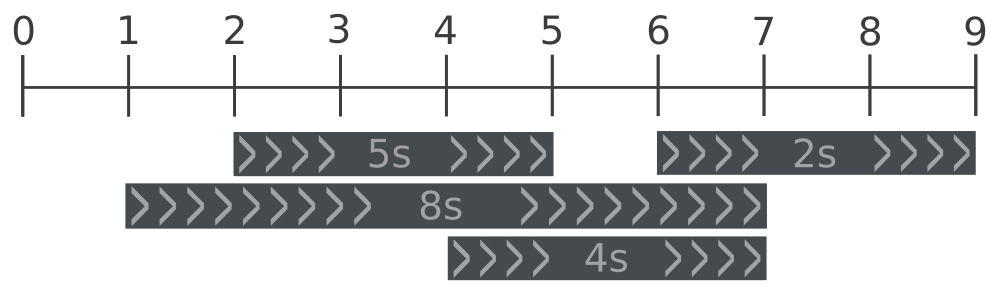
\includegraphics[width=0.5\textwidth]{sample1}
\caption{Ett av två optimala sätt att klippa i exempelfall 1}
\end{figure}
